\documentclass[a4paper]{article}

\usepackage{a4wide}
\usepackage[utf8]{inputenc}
\usepackage[ngerman]{babel}
\usepackage{fancyhdr}
\usepackage{graphicx}
\usepackage[parfill]{parskip}
\pagestyle{fancy}
\topmargin -5mm
\headheight 20mm

% include logo in document head
\chead{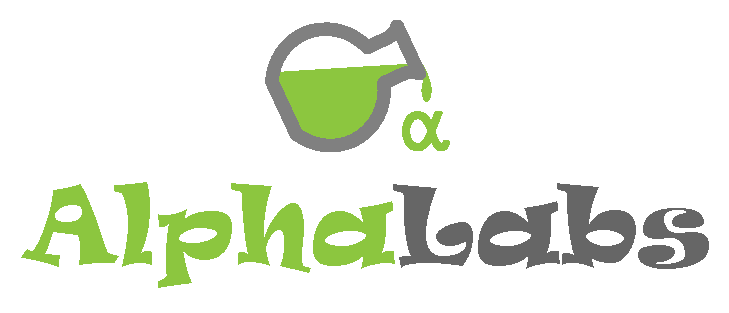
\includegraphics[width=50mm]{logo.pdf}}

% footer
\lfoot{AlphaLabs, Gruppe 1}
\cfoot{}
\rfoot{Name 1, Name 2, Name 3}

% bottom line
\renewcommand{\footrulewidth}{0.4pt}

% change standard font
\usepackage[T1]{fontenc}
\newcommand{\changefont}[3]{
\fontfamily{#1} \fontseries{#2} \fontshape{#3} \selectfont}


\begin{document}
\changefont{cmss}{m}{n} %computer modern sans serif

\begin{center}
\textbf{\huge Spielkonzeptvorschläge}
\end{center}


\vspace{5mm}

\textbf{Name:} GeoMatch\\
\textbf{Genres:} Point ‘n Klick, Geographie, Lernspiel\\
\textbf{Zielgruppe:} Wir wollen insbesondere jüngere Schüler im Altersbereich von 8-14 ansprechen, aber auch für ältere Benutzer, die ihr Geographie-Wissen auffrischen wollen.\\
\textbf{Beschreibung:}\\
Worum geht es?\\
Die Spieler können ihr Wissen über ausgewählte Objekte wie Städte/Länder/Regionen/Berge/Flüsse erweitern und testen können, indem diese Objekte mit ihrer geographischen Lage sowie weiterer Merkmale wie z.B. der Landesflaggen, passender Speisen, spezieller Bräuche, Nationalhymnen und weiterer, verknüpft werden.\\
Wie setzen wir das um?\\
Man hat die Möglichkeit sich auf bestimmte Kontinente zu beschränken oder aber die komplette Welt zu wählen und sich Objekte und Merkmale anzusehen und einzuprägen.
Im Folgenden versucht man mit verschiedenen Minispielen, die Objekte ihrer Lage oder ihren Merkmalen zuzuordnen und dies in möglichst kurzer Zeit, mit wenig Versuchen und wenigen Tipps.\\
Minispiel-Ideen:\\
\begin{enumerate}
\item Standort von Objekten muss auf einer Karte möglichst genau getroffen werden
\item Einfaches Memory
\item „Wer oder was bin ich“ – Spiel (anhand von möglichst wenig gegebenen Merkmalen auf ein Objekt kommen) 
\end{enumerate}

\vspace{1cm}

\textbf{Name:} Circle of Waste\\
\textbf{Genres:} Point 'n Click, Lernspiel\\
\textbf{Zielgruppe:} Didaktische Mittel und graphische Oberflaeche sind auf Kinder von 8-14 Jahren ausgerichtet.\\
\textbf{Beschreibung:} \\
Das Lernspiel \textit{Circle of Waste} soll Kindern auf spielerische Weise den Weg des Mülls in unserer Gesellschaft zeigen. Dies fängt beim verantwortungsvollen Einkaufen an und geht bis zur Wiederverwendung von Verpackungsmaterialien durch Recycling. Durch verschiedene Minispiele auf dem Weg sollen die korrekte Mülltrennung erlernt, Hintergrundinformationen zu Müllverwertung und Recycling vermittelt und das Bewusstsein für die Umwelt gestärkt werden. Die Spielerin oder der Spieler wird durch das Spiel hinweg von einem Maskottchen begleitet (z.B. ein Hund). Eventuell wird es auch einen "Bösewicht" geben, welcher Müll auf falsche Art und Weise entsorgt.\\
Mögliche Minispiele sind Quizze, Memory, ein Zuordnungsspiel per Drag'n'Drop oder eine Art Auffangspiel, in dem Müll richtig sortiert werden muss.

\end{document}
